%xelatex
\documentclass[12pt]{extreport}
%\documentclass[14pt]{extreport}

\usepackage{listings}
%\usepackage{verbatim}
\usepackage[T2A]{fontenc}
\usepackage[english,ukrainian]{babel}
\usepackage{mathspec}
\setallmainfonts{Nimbus Roman}
\usepackage{graphicx}
\usepackage{caption}
\usepackage{subcaption}
\usepackage[a4paper,margin=0.5in]{geometry}
\usepackage{tikz}
\usetikzlibrary{calc,positioning,shapes.geometric,shapes.symbols,shapes.misc}
\usepackage{indentfirst}
\usepackage{moreverb}
\usepackage{subfiles}

\lstset{
  basicstyle=\ttfamily,
  columns=fullflexible,
  breaklines=true,
  postbreak=\raisebox{0ex}[0ex][0ex]{\color{red}$\hookrightarrow$\space}
}

\begin{document}

\subfile{title.tex}

%{\fontsize{18}{20.7}\selectfont \textbf{Лабораторна робота №1}}
%{\fontsize{14}{16.1}\selectfont
\subsubsection*{Мета роботи}
Ознайомитися із особливостями застосування функцій у мові С.

\bigskip
\subsubsection*{Завдання № 1}
Виконати завдання, наведені нижче. Ввід-вивд даних та виконання інших
окремих логічних дій необхідно реалізувати в окремих функціях. У головній
функції необхідно виконувати лише їх виклик. Використання глобальних
змінних не допускається. Інформація повинна передаватися у функції лише за
допомогою параметрів.

Обчислити означений інтеграл функції: $1 + \cos^2x$, на інтервалі [0,\pi],
використовуючи формулу лівих прямокутників. Крок вводити з клавіатури.

\bigskip
Схема алгоритму зображена на рис. 1.

\begin{figure}[h]
\begin{subfigure}{.5\textwidth}
	\centering
	\subfile{fch.tex}
	\caption{Схема алгоритму для першого завдання}
\end{subfigure}
\hfill
\begin{subfigure}{.5\textwidth}
	\centering
	\subfile{fchint.tex}
	\caption{функція обчислення інтегралу для першого завдання}
\end{subfigure}
	\caption{}
\end{figure}
\subsubsection*{Програмний код до першого завдання}

Функція для обчислення інтегралу:
\begin{lstlisting}[frame=single]
#include <stdio.h>
#include <math.h>

double integr(double N){
	double y=0.0, x=0.0, integral = 0.0;

	while(x<=3.1415){
		y = 1 + pow(cos(x), 2);
		integral = integral + N * y;
		x=x+N;
	}
	printf("Integral on segment [-1.0,3.1415], calculated using the left rectangle method"
		"with step %lf: %lf\n", N, integral);
	return integral;
}
\end{lstlisting}

Головна функція та функція, відведена для вводу значення кроку:
\begin{lstlisting}[frame=single]
#include <stdio.h>
#include "integr.c"

double func(){
	double N;
	scanf("%lf", &N);
	return N;
}

int main(){

	integr(func());
}

\end{lstlisting}

Вивід:

\begin{lstlisting}
Integral on segment [-1.0,3.1415], calculated using the left rectangle methodwith step 0.010000: 4.729204
\end{lstlisting}

\subsubsection*{Завдання № 2}
Виконати аналіз текстового файлу (текст довільний). Назва текстового файлу
та інші вхідні дані передаються в програму через аргументи функції \texttt{main()}.

Визначити кількість знаків з пробілами і без пробілів.

\bigskip
Схема алгоритму зображена на рис. \ref{task2}

\begin{figure}[h]
	\begin{subfigure}[b]{.3\textwidth}
	\centering
	\subfile{fch2.tex}
		\caption{Схема програми}
	\end{subfigure}
	\hfill
	\begin{subfigure}[b]{.3\textwidth}
	\centering
		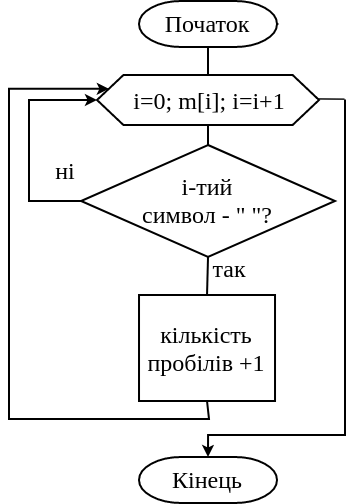
\includegraphics[width=.9\textwidth]{fch/fchc.png}
		\caption{Схема функції обчислення кількості символів без пробілів}
	\end{subfigure}
	\hfill
	\begin{subfigure}[b]{.3\textwidth}
	\centering
	\subfile{fch/fchr.tex}
		\caption{ввідна функція}
	\end{subfigure}
	\caption{Схема алгоритму для другого завдання}
	\label{task2}
\end{figure}

\newpage
\subsubsection*{Програмний код до другого завдання}
\begin{lstlisting}[frame=single]
#include <stdio.h>
#include <string.h>

int countsp(char m[]){
		int count=0;

		for(int i=0; m[i]; i++){
			if(m[i]==' ')
				count++;
		}

		int wospaces = strlen(m)-1-count;

		return wospaces;
}

int write(int wsp){
	printf("with spaces: %d\n", wsp);
}

int writewo(int wosp){
	printf("without spaces: %d\n", wosp);
}

int read(char *arg[]){
	FILE *fp = fopen(arg[1], arg[2]);

		char m[400];
		fgets(m, 400, fp);

	fclose(fp);
	writewo(countsp(m));
	return strlen(m)-1;
}

int main(int argc, char *argv[]){

	write(read(argv));
	return 0;
}
\end{lstlisting}

Вивід:
\begin{lstlisting}
[sh@host ~/UNI/c/progs/lab7/t2]$ ./main text "r"
without spaces: 240
with spaces: 279
\end{lstlisting}

\subsubsection*{Висновок:}
У цій лабораторній роботі я ознайомився з особливостями
застосування функцій у мові C.

\end{document}
